\documentclass[12pt]{article}
\usepackage{graphicx}
\usepackage[a4paper, margin=1in]{geometry}
\usepackage{import}
\usepackage{amsmath}
\usepackage{xcolor}
\usepackage{fancyhdr}
\usepackage{enumitem}
\usepackage{tcolorbox}
\usepackage{float}
\usepackage{url}
\usepackage{hyperref}
\usepackage{multirow}
\usepackage{array}
\usepackage{tikz}
\usetikzlibrary{shapes.geometric, arrows.meta, positioning, calc}
\usepackage{standalone}
\usepackage{subcaption}

\definecolor{linegray}{RGB}{128, 128, 128}

% lstlisting settings for Verilog
\usepackage{listings}
\usepackage{courier}
\lstdefinelanguage{Verilog}{
    keywords={input, output, assign, wire, reg, always, begin, end, case, endcase, default, if, else, posedge, negedge, parameter, initial, timescale, \$display, \$monitor, \$finish},
    keywordstyle=\color{blue}\bfseries,
    identifierstyle=\color{black},
    % comment=[l={//}],
    commentstyle=\color{green}\itshape,
    stringstyle=\color{red},
    basicstyle=\footnotesize\ttfamily, % Courier font
    morekeywords=[2]{module,endmodule},
    keywordstyle=[2]{\color{purple}\bfseries},
    numbers=left,
    numberstyle=\tiny\color{linegray},
    stepnumber=1,
    numbersep=8pt,
    backgroundcolor=\color{gray!10},
    frame=single,
    rulecolor=\color{gray!60},
    tabsize=2,
    showstringspaces=false,
    breaklines=true,
    breakatwhitespace=true,
    captionpos=b
}

\pagestyle{fancy}
\fancyhf{}
\renewcommand{\headrulewidth}{0.5pt}
\setlength{\headheight}{15pt}
\rhead{\textbf{16-bit MIPS Processor Design}}
\lhead{CSE 431 - Advanced Computer Architecture}

\fancyfoot[R]{MIPS-16 \textbar \ \textbf{\thepage}}
\renewcommand{\footrulewidth}{0.5pt}

\setlist[enumerate]{label=\arabic*., font=\itshape, leftmargin=1.5cm}

\newtcolorbox{answerbox}{
    colback=gray!5,
    colframe=gray!60,
    boxrule=0.4pt,
    arc=4pt,
    left=6pt,
    right=6pt,
    top=6pt,
    bottom=6pt,
    width=\linewidth,
    before skip=6pt,
    after skip=12pt,
}

\begin{document}

\linespread{1.5}\selectfont
\import{./}{cover}

\newpage
\tableofcontents
\newpage
\listoffigures
\listoftables
\lstlistoflistings
\newpage

\section{Abstract}
\vspace{0.3cm}
This technical report presents the design and implementation of a \textbf{16-bit MIPS} (Million Instructions Per Second) processor, in both \textbf{single-cycle} and \textbf{pipelined architectures}. The report details the design specifications, including the \textbf{instruction set architecture (ISA)} and \textbf{control signal encoding}. It also includes \textbf{datapath schematics} for both architectures along with \textbf{waveform simulations} for testing and verification. Finally, a \textbf{performance comparison} with analysis summarizes the advantages and trade-offs between the two designs.

\vspace{0.5cm}

\vspace{0.5cm}

\section{Introduction}
\vspace{0.3cm}
MIPS architecture is a RISC (Reduced Instruction Set Computer) architecture that is widely used in computer engineering education and research. The 16-bit MIPS processor introduced in this report is a simplified version of the standard MIPS architecture. The processor supports very basic set of instructions with minimal specifications. The main differences between both processor will be highlighted throughout the report.

\subsection{Objectives}
\vspace{0.2cm}
The primary objectives of this project are:
\begin{itemize}
    \item \textbf{Design and implement} a simple 16-bit MIPS processor in both single-cycle and pipelined architectures.
    \item \textbf{Simulate and verify} both processor designs using simple tests with waveform analysis.
    \item \textbf{Compare the performance} of single-cycle and pipelined architectures.
    \item \textbf{Provide insights} into the trade-offs between single-cycle and pipelined designs.
    \item \textbf{Document the design process, specifications, and performance analysis} in this technical report.
\end{itemize}

\vspace{0.3cm}

\subsection{Development Environment}
\vspace{0.2cm}
The development environment for this project includes:
\begin{itemize}
    \item Hardware Description Language (HDL): \textbf{Verilog}
    \item Compilation Tool: \textbf{Quartus (Web Edition)}
    \item Simulation Tool: \textbf{ModelSim} (included with Quartus)
\end{itemize}

\vspace{0.5cm}

\section{Design Specifications}
\vspace{0.3cm}

\subsection{Memory Organization}
\vspace{0.2cm}
The 16-bit MIPS processor utilizes two separate memory interfaces for instruction and data memory, respectively. This eliminates \textit{structural hazards}\footnote{Structural hazards occur when multiple instructions need to use the same resources simultaneously} and allow for simultaneous instruction fetch and data access in the pipelined architecture.

While the standard MIPS architecture uses the Big-Endian format for memory storage, this 16-bit MIPS processor employs the Little-Endian format. In Little-Endian format, the least significant byte (LSB) is stored at the lowest memory address, while the most significant byte (MSB) is stored at the highest memory address. This choice simplifies certain operations and aligns with common practices in various computing systems.
\begin{figure}[H]
    \centering
    \includegraphics[width=0.8\linewidth]{assets/32bit-Endianess.pdf}
    \caption{Illustration of Little-Endian and Big-Endian memory layouts. Source: \href{https://commons.wikimedia.org/wiki/File:32bit-Endianess.svg}{Wikimedia Commons}}
    \label{fig:endianess_illustration}
\end{figure}

\vspace{0.3cm}

\subsubsection{Instruction Memory}
\vspace{0.2cm}
The instruction memory is a \textit{byte-addressable}\footnote{Meaning that each location stores one byte (8 bits) of data}, read-only memory module with \textbf{64 bytes} of storage (addresses 0x00 to 0x3F). It is implemented in \textbf{little-endian} format and stores program instructions.

\begin{figure}[H]
    \centering
    \begin{tabular}{r@{\hspace{0.5em}}|>{\centering\arraybackslash}p{3cm}|}
        \cline{2-2}
        0x00 & 0x00 \\ \cline{2-2}
        0x01 & 0x81 \\ \cline{2-2}
        0x02 & 0x42 \\ \cline{2-2}
        0x03 & 0x81 \\ \cline{2-2}
    \end{tabular}

    \vspace{1em}
    \begin{tabular}{r@{\hspace{0.5em}}>{\centering\arraybackslash}p{3cm}}
         & $\vdots$
    \end{tabular}
    \vspace{1em}

    \begin{tabular}{r@{\hspace{0.5em}}|>{\centering\arraybackslash}p{3cm}|}
        \cline{2-2}
        0x3F & 0x00 \\ \cline{2-2}
    \end{tabular}
    \caption{Instruction Memory Layout (64 bytes)}
    \label{fig:instruction_memory}
\end{figure}

\vspace{0.3cm}

\subsubsection{Data Memory}
\vspace{0.2cm}
Like the instruction memory, the data memory is also a byte-addressable, little-endian memory module with \textbf{64 bytes} of storage. It supports both read and write operations. \autoref{fig:data_memory} shows an abstract representation example of the memory layout.

\begin{figure}[H]
    \centering
    \begin{tabular}{r@{\hspace{0.5em}}|>{\centering\arraybackslash}p{3cm}|}
        \cline{2-2}
        0x00 & 0x12 \\ \cline{2-2}
        0x01 & 0x02 \\ \cline{2-2}
        0x02 & 0x22 \\ \cline{2-2}
        0x03 & 0x20 \\ \cline{2-2}
    \end{tabular}

    \vspace{1em}
    \begin{tabular}{r@{\hspace{0.5em}}>{\centering\arraybackslash}p{3cm}}
         & $\vdots$
    \end{tabular}
    \vspace{1em}

    \begin{tabular}{r@{\hspace{0.5em}}|>{\centering\arraybackslash}p{3cm}|}
        \cline{2-2}
        0x3F & 0x00 \\ \cline{2-2}
    \end{tabular}
    \caption{Data Memory Layout (64 bytes)}
    \label{fig:data_memory}
\end{figure}

\vspace{0.3cm}

\textbf{Key Feature:}
\vspace{0.2cm}
\begin{itemize}[itemsep=0.1cm]
    \item Supports both read and write operations.
    \item Byte-addressable with little-endian format.
    \item \textbf{Synchronous write:} Data is written to memory on the rising edge of the clock when \texttt{MemWrite = 1} signal is asserted.
    \item \textbf{Asynchronous read:} Data can be read from memory at any time without needing for a read signal.
\end{itemize}

\vspace{0.3cm}

\subsubsection{Memory Interfaces}
\vspace{0.2cm}
Both memories follow the following interface specifications:

\begin{table}[H]
    \centering
    \begin{tabular}{|l|c|}
        \hline
        \textbf{Parameter} & \textbf{Specification} \\ \hline
        Data Width         & 16-bit                 \\ \hline
        Instruction Width  & 16-bit                 \\ \hline
        Address Width      & 16-bit                 \\ \hline
        Memory Model       & Byte-Addressable       \\ \hline
    \end{tabular}
    \caption{Design Specifications}
    \label{tab:design_specs}
\end{table}

\textbf{Instruction Memory Interface:}

\begin{figure}[H]
    \centering
    \includestandalone{diagrams/instruction_memory}
    \caption{Instruction Memory Block Diagram}
    \label{fig:instruction_memory_block}
\end{figure}

\textbf{Data Memory Interface:}

\begin{figure}[H]
    \centering
    \includestandalone{diagrams/data_memory}
    \caption{Data Memory Block Diagram}
    \label{fig:data_memory_block}
\end{figure}

\vspace{0.5cm}

\subsection{Instruction Set Architecture (ISA)}
\vspace{0.2cm}
The 16-bit MIPS processor supports a simplified ISA with a minimal set of instructions. The processor implements a 16-bit instruction word with support for R-Type and I-Type instructions, along with branch instructions for the single-cycle.

The instruction formats, supported instructions, register file, control signals, and ALU control encoding are detailed in the following subsections.

\vspace{0.3cm}

% R-Type and I-Type instruction formats
\subsubsection{Instruction Formats}
\vspace{0.2cm}

\textbf{R-Type Instruction Format:}

\begin{figure}[H]
    \centering
    \includestandalone[width=0.6\linewidth]{diagrams/r-type_format}
    \caption{R-Type Instruction Format (16-bit)}
    \label{fig:r_type_format}
\end{figure}

\vspace{0.4cm}

\textbf{I-Type Instruction Format:}

\begin{figure}[H]
    \centering
    \includestandalone[width=0.6\linewidth]{diagrams/i-type_format}
    \caption{I-Type Instruction Format (16-bit)}
    \label{fig:i_type_format}
\end{figure}

\vspace{0.5cm}

% Opcode table (available instructions)
\subsubsection{Supported Instructions}
\vspace{0.2cm}
The 16-bit MIPS processor supports the following instructions:
\begin{table}[H]
    \centering
    \begin{tabular}{|l|c|c|c|l|}
        \hline
        \textbf{Instruction} & \textbf{Format} & \textbf{Opcode} & \textbf{Funct} & \textbf{Description}             \\ \hline
        \multicolumn{5}{|c|}{\textit{R-Type Instructions (Opcode = 0000)}}                                           \\ \hline
        \textbf{AND}         & R               & 0000            & 000            & rd = rs \& rt                    \\ \hline
        \textbf{OR}          & R               & 0000            & 001            & rd = rs $\mid$ rt                \\ \hline
        \textbf{ADD}         & R               & 0000            & 010            & rd = rs + rt                     \\ \hline
        \textbf{XOR}         & R               & 0000            & 011            & rd = rs $\oplus$ rt              \\ \hline
        \textbf{NOR}         & R               & 0000            & 100            & rd = $\sim$(rs $\mid$ rt)        \\ \hline
        \textit{Reserved}    & R               & 0000            & 101            & \textit{Reserved for future use} \\ \hline
        \textbf{SUBTRACT}    & R               & 0000            & 110            & rd = rs - rt                     \\ \hline
        \textbf{SLT}         & R               & 0000            & 111            & rd = (rs $<$ rt) ? 1 : 0         \\ \hline
        \multicolumn{5}{|c|}{\textit{I-Type Instructions}}                                                           \\ \hline
        \textbf{ADDI}        & I               & 0001            & ---            & rt = rs + SignExt(Imm)           \\ \hline
        \textbf{SUBI}        & I               & 0010            & ---            & rt = rs - SignExt(Imm)           \\ \hline
        \textbf{LW}          & I               & 1000            & ---            & rt = Mem[rs + SignExt(Imm)]      \\ \hline
        \textbf{SW}          & I               & 1010            & ---            & Mem[rs + SignExt(Imm)] = rt      \\ \hline
        \textbf{BEQ}         & I               & 1100            & ---            & if (rs == rt) PC += SignExt(Imm) \\ \hline
    \end{tabular}
    \caption{Supported Instructions}
    \label{tab:supported_instructions}
\end{table}

\vspace{0.5cm}

% Registers table
\subsection{Register File}
\vspace{0.2cm}
\subsubsection{Register File Specifications}
\vspace{0.2cm}
The register file is responsible for storing and providing access to the processor's registers. It contains 8 general-purpose registers, each is 16-bit wide. The register \texttt{\$0} is hardwired to the constant value 0. The remaining registers (\texttt{\$1} to \texttt{\$7}) can be used for general-purpose data storage and manipulation.
\begin{table}[H]
    \centering
    \begin{tabular}{|l|c|l|}
        \hline
        \textbf{Register} & \textbf{Number} & \textbf{Description}       \\ \hline
        \$0               & 000             & Constant value 0           \\ \hline
        \$v0              & 001             & General-purpose register 1 \\ \hline
        \$a0              & 010             & General-purpose register 2 \\ \hline
        \$a1              & 011             & General-purpose register 3 \\ \hline
        \$t0              & 100             & General-purpose register 4 \\ \hline
        \$t1              & 101             & General-purpose register 5 \\ \hline
        \$s0              & 110             & General-purpose register 6 \\ \hline
        \$s1              & 111             & General-purpose register 7 \\ \hline
    \end{tabular}
    \caption{Available Registers}
    \label{tab:register_file}
\end{table}

\vspace{0.3cm}

\subsubsection{Register File Interface}
\vspace{0.2cm}

\begin{figure}[H]
    \centering
    \includestandalone{diagrams/reg_file}
    \caption{Register File Block Diagram}
    \label{fig:register_file_block}
\end{figure}

\vspace{0.5cm}

% Control Signals table for every instruction
\subsection{Control Signals}
\vspace{0.2cm}
\subsubsection{Control Unit}
\vspace{0.2cm}
The control unit generates the necessary control signals based on the \textbf{opcode} and \textbf{funct} fields of the instruction. These control signals dictate the operation of various components within the processor, such as the ALU, register file, and memory. The control unit interface is illustrated in \autoref{fig:control_unit_block}.

\begin{figure}[H]
    \centering
    \includestandalone{diagrams/control_unit}
    \caption{Control Unit Block Diagram}
    \label{fig:control_unit_block}
\end{figure}

\vspace{0.3cm}

\subsubsection{Control Signals Truth Table}
\vspace{0.2cm}
\begin{table}[H]
    \centering
    \small
    \begin{tabular*}{\linewidth}{|l|@{\extracolsep{\fill}}>{\centering\arraybackslash}m{1.2cm}|>{\centering\arraybackslash}m{1.2cm}|>{\centering\arraybackslash}m{1.5cm}|>{\centering\arraybackslash}m{1.5cm}|>{\centering\arraybackslash}m{1.2cm}|>{\centering\arraybackslash}m{1.5cm}|>{\centering\arraybackslash}m{1.3cm}|}
        \hline
        \textbf{Instruction} & \textbf{Reg Dst} & \textbf{Branch} & \textbf{Mem To Reg} & \textbf{Mem Write} & \textbf{ALU Src} & \textbf{Reg Write} & \textbf{ALU Ctrl} \\ \hline
        \textbf{R-Type}      & 1                & 0               & 0                   & 0                  & 0                & 1                  & funct             \\ \hline
        \textbf{ADDI}        & 0                & 0               & 0                   & 0                  & 1                & 1                  & 010               \\ \hline
        \textbf{SUBI}        & 0                & 0               & 0                   & 0                  & 1                & 1                  & 110               \\ \hline
        \textbf{LW}          & 0                & 0               & 1                   & 0                  & 1                & 1                  & 010               \\ \hline
        \textbf{SW}          & X                & 0               & X                   & 1                  & 1                & 0                  & 010               \\ \hline
        \textbf{BEQ}         & X                & 1               & X                   & 0                  & 0                & 0                  & 110               \\ \hline
    \end{tabular*}
    \caption{Instructions Control Signals}
    \label{tab:control_signals}
\end{table}

Note that `X' indicates a \textit{``don't care''}\footnote{A condition where the value of the control signal does not affect the operation of the instruction.} condition for that particular control signal.

\vspace{0.5cm}

% ALUCtrl table
\subsection{ALU Control Encoding}
\vspace{0.2cm}
The 3-bit \texttt{ALUCtrl} signal specifies the operation to be performed by the ALU. The encoding is as follows:
\begin{table}[H]
    \centering
    \begin{tabular}{|c|l|l|}
        \hline
        \textbf{ALUCtrl} & \textbf{Operation} & \textbf{Description}      \\ \hline
        000              & AND                & Bitwise AND               \\ \hline
        001              & OR                 & Bitwise OR                \\ \hline
        010              & ADD                & Addition                  \\ \hline
        011              & XOR                & Bitwise XOR               \\ \hline
        100              & NOR                & Bitwise NOR               \\ \hline
        101              & ---                & Reserved                  \\ \hline
        110              & SUBTRACT           & Subtraction               \\ \hline
        111              & SLT                & Set on Less Than (signed) \\ \hline
    \end{tabular}
    \caption{ALU Control Signal Encoding}
    \label{tab:alu_ctrl}
\end{table}
Note that ALUCtrl takes the same value as the \texttt{funct} field for R-Type instructions (see \autoref{tab:supported_instructions}).

\vspace{0.5cm}

\section{Datapath Schematics}
\vspace{0.3cm}
\subsection{Single-Cycle Datapath}
\vspace{0.2cm}
The single-cycle architecture executes each instruction in one clock cycle. The entire datapath is designed to accommodate the longest instruction execution time, which may lead to inefficiencies for simpler instructions.

\subsubsection{Datapath Modules}
\vspace{0.2cm}
\begin{itemize}[itemsep=0.1cm]
    \item \textbf{Program Counter (PC):} Holds the address of the next instruction to be fetched.
    \item \textbf{Instruction Memory (IM):} Stores the program instructions.
    \item \textbf{Register File (RF):} Holds the general-purpose registers.
    \item \textbf{Control Unit:} Generates control signals based on the opcode of the instruction.
    \item \textbf{Arithmetic Logic Unit (ALU):} Performs arithmetic and logical operations.
    \item \textbf{Sign Extend:} Extends 6-bit immediate values to 16 bits.
    \item \textbf{Data Memory (DM):} Stores data for load and store instructions.
    \item \textbf{2-to-1 Multiplexers:} Selects between two data sources based on control signals.
\end{itemize}

\vspace{0.3cm}

\subsubsection{Single-Cycle Datapath Schematic}
\vspace{0.2cm}

\begin{figure}[H]
    \centering
    \includegraphics[width=\linewidth]{assets/processorSC.pdf}
    \caption{Single-Cycle Datapath Schematic}
    \label{fig:single_cycle_datapath}
\end{figure}

\vspace{0.5cm}

\subsection{Pipelined Datapath}
\vspace{0.2cm}
The pipelined architecture divides instruction execution into multiple stages, allowing for overlapping execution of instructions. This improves overall throughput but introduces complexity in handling hazards. It uses the same modules as the single-cycle architecture, but with additional pipeline registers between stages. For simplicity, no branch prediction or hazard detection mechanisms are implemented in this design.

\subsubsection{Pipeline Stages}
\vspace{0.2cm}
\begin{itemize}[itemsep=0.1cm]
    \item \textbf{Instruction Fetch (IF):} Fetches the instruction from instruction memory.
    \item \textbf{Instruction Decode (ID):} Decodes the instruction and reads registers.
    \item \textbf{Execute (EX):} Performs ALU operations or calculates addresses.
    \item \textbf{Memory Access (MEM):} Accesses data memory for load/store instructions.
    \item \textbf{Write Back (WB):} Writes results back to the register file.
\end{itemize}

\vspace{0.2cm}

To separate these stages, pipeline registers are used to hold intermediate values between stages. This ensures that each stage can operate independently and concurrently. The registers used are as follows:

\vspace{0.2cm}

\begin{itemize}[itemsep=0.1cm]
    \item \textbf{IF/ID Register:} Holds the instruction fetched from instruction memory between the IF and ID stages.
    \item \textbf{ID/EX Register:} Holds decoded instruction data, control signals, register values, and immediate values between the ID and EX stages.
    \item \textbf{EX/MEM Register:} Holds the ALU result, memory write data, control signals, and destination register between the EX and MEM stages.
    \item \textbf{MEM/WB Register:} Holds data from memory, ALU result, control signals, and destination register between the MEM and WB stages.
\end{itemize}

\vspace{0.3cm}

\subsubsection{Pipelined Datapath Schematic}
\vspace{0.2cm}
\begin{figure}[H]
    \centering
    \includegraphics[width=\linewidth]{assets/processorPipe.pdf}
    \caption{Pipelined Datapath Schematic}
    \label{fig:pipelined_datapath}
\end{figure}

\vspace{0.5cm}

\section{Waveform Simulation and Verification}
\vspace{0.3cm}
Both processor designs were simulated and verified using \texttt{Quartus} with the help of \texttt{ModelSim}. Vector Waveform Files (VWF) were created to test the functionality of each processor design. The following subsections present the test instructions and the waveform results for both architectures.

The data memory is initialized to contain the following values before simulation:
\begin{table}[H]
    \centering
    \begin{tabular}{|c|c|}
        \hline
        \textbf{Address} & \textbf{Value} \\ \hline
        0x00             & 0x12           \\ \hline
        0x01             & 0x02           \\ \hline\hline
        0x02             & 0x22           \\ \hline
        0x03             & 0x20           \\ \hline
    \end{tabular}
    \caption{Initial Data Memory Values}
    \label{tab:initial_data_memory}
\end{table}
Meaning, \texttt{Mem[0] = 0x0212} and \texttt{Mem[2] = 0x2022}, since it is a little-endian architecture. The rest of the memory is initialized to 0x00. The following sections detail the test instructions and waveform results for both processor architectures. Note that the introduced codes are assembly instructions that were converted to machine code (binary) before being loaded into the instruction memory.

\vspace{0.4cm}

\subsection{Single-Cycle Verification}
\vspace{0.2cm}
\subsubsection{Single-Cycle Test Instructions}
\vspace{0.2cm}
The following assembly code was used to test the single-cycle processor:
\lstinputlisting[language=Verilog, caption={Single-Cycle Test Instructions}, label={lst:sc_instructions}]{assets/codes/SC_instructions.asm}

\vspace{0.3cm}

\subsubsection{Single-Cycle Simulation Waveform}
\vspace{0.2cm}
\begin{figure}[H]
    \centering
    \begin{minipage}{\linewidth}
        \centering
        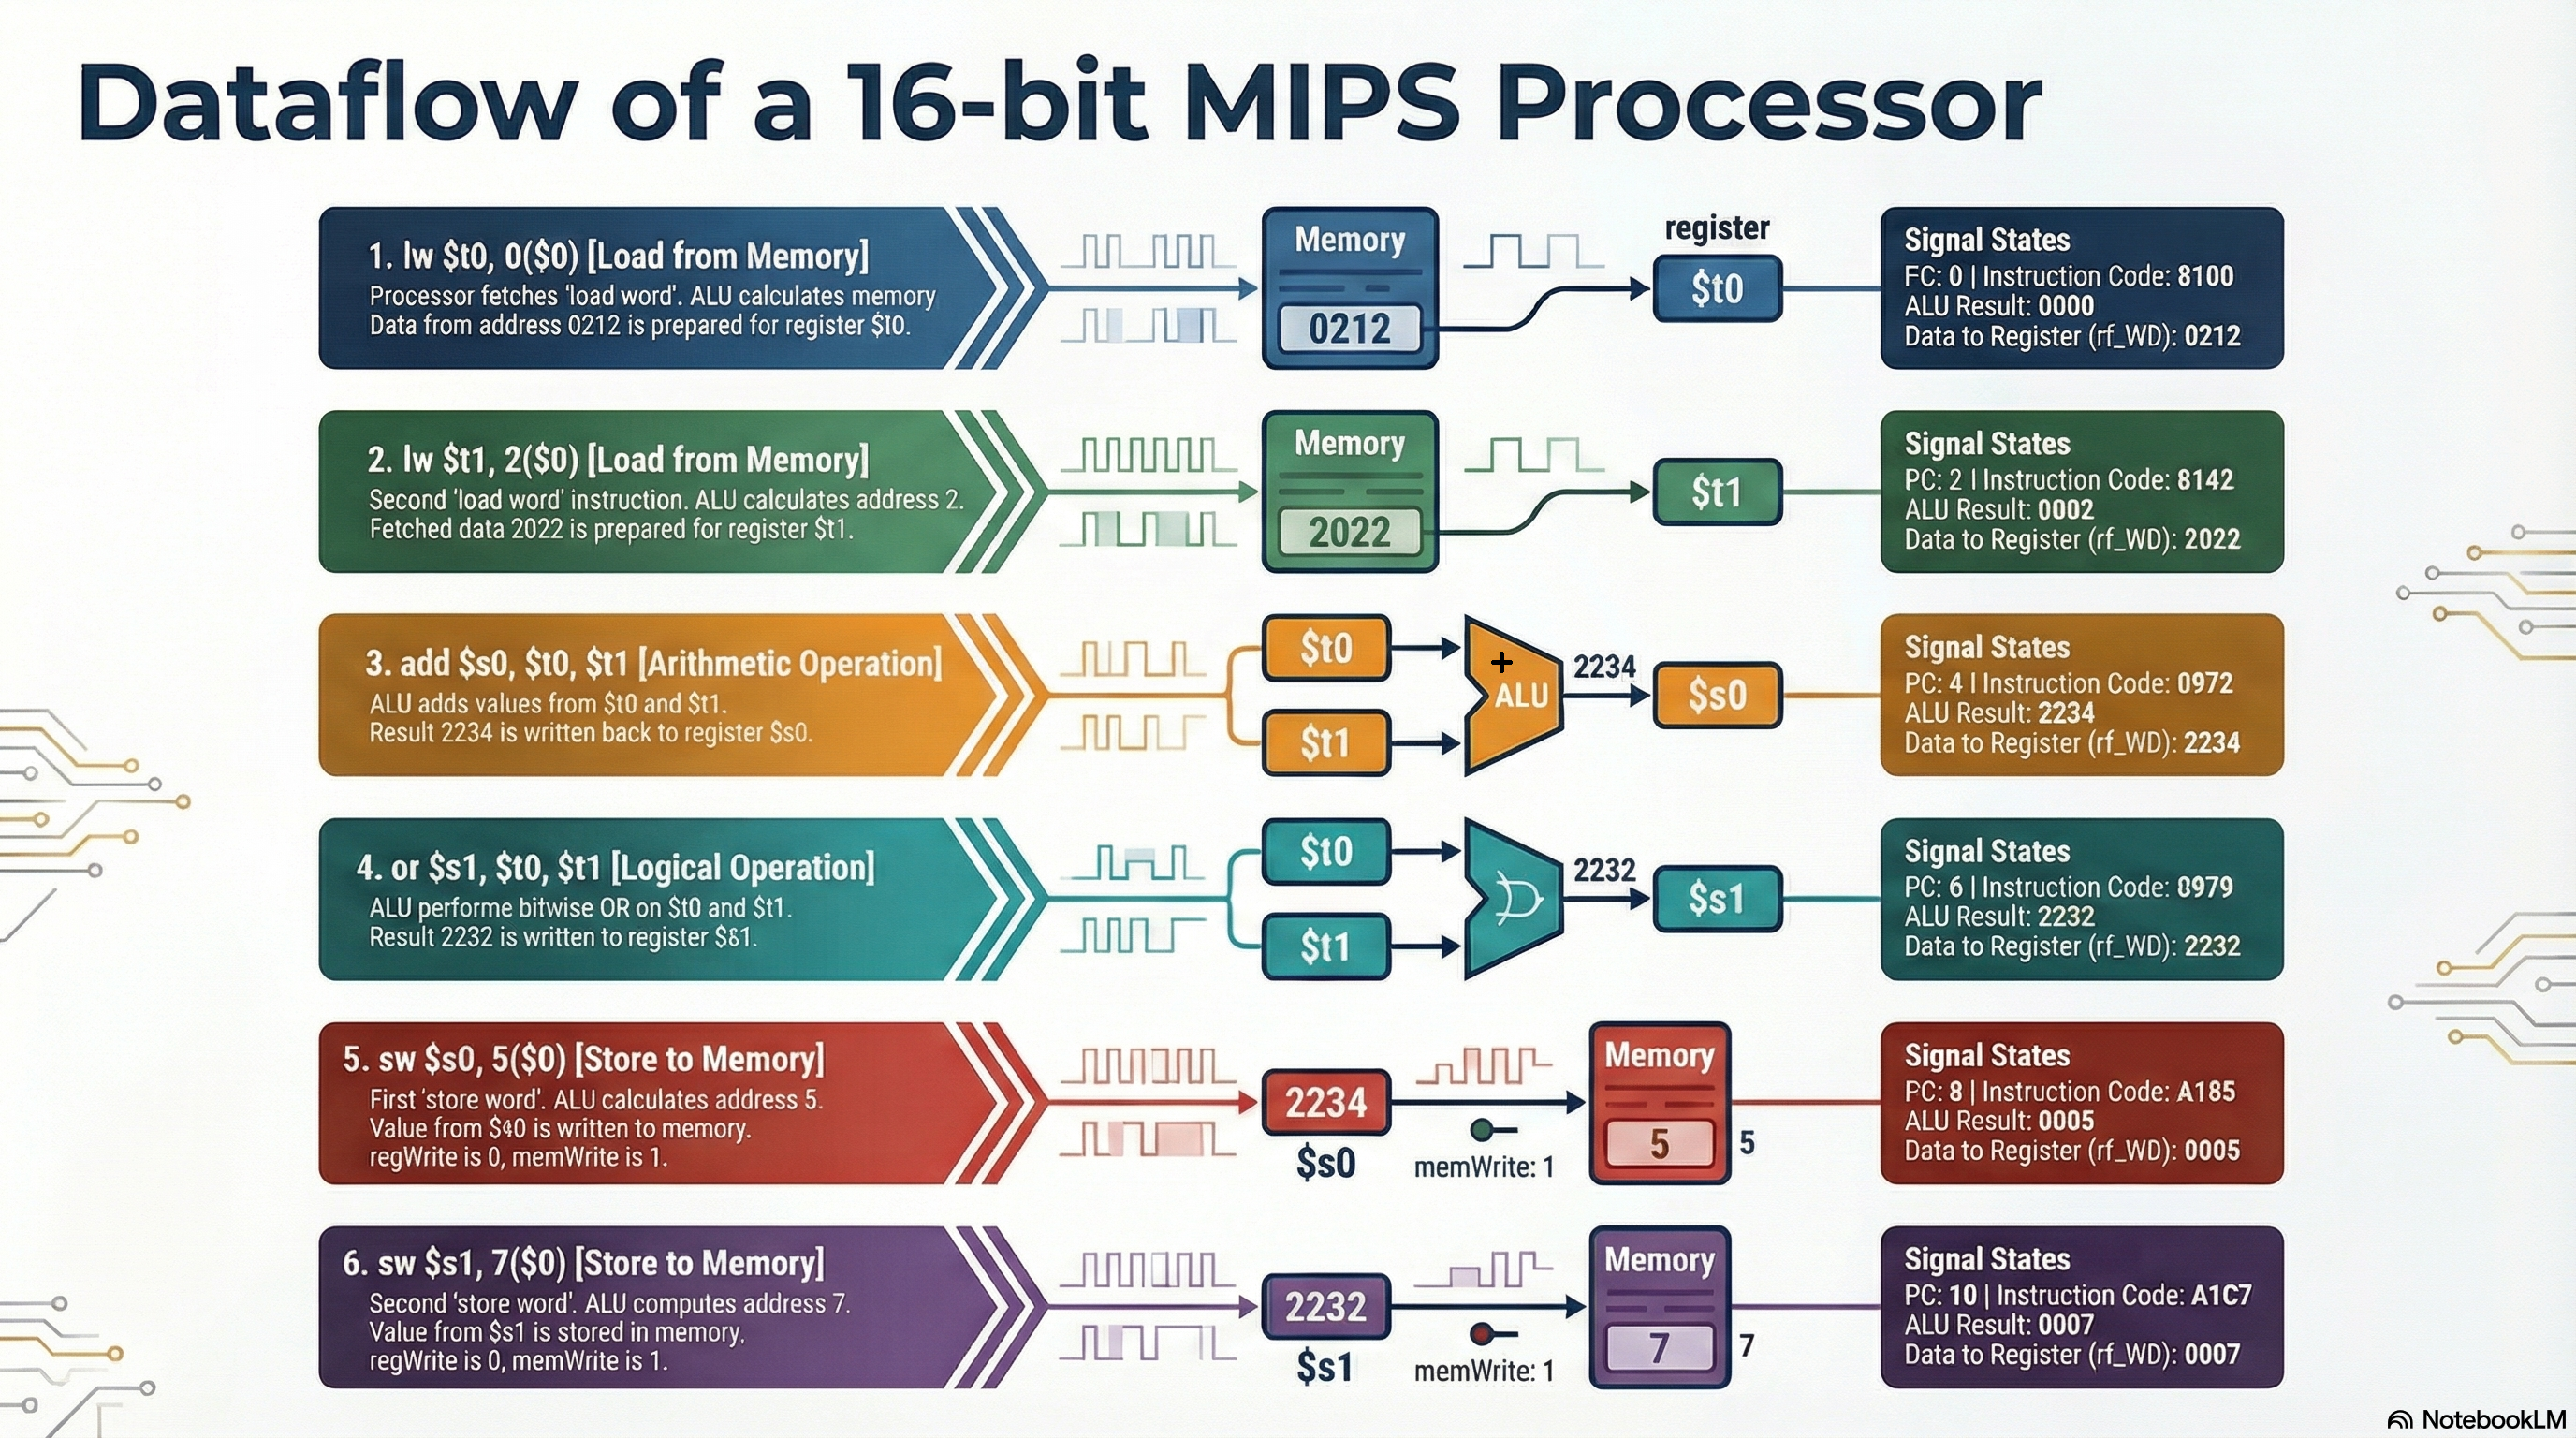
\includegraphics[width=\linewidth]{assets/WaveformSC.jpg}
        \subcaption{Original waveform}
    \end{minipage}

    \vspace{1em}

    \begin{minipage}{\linewidth}
        \centering
        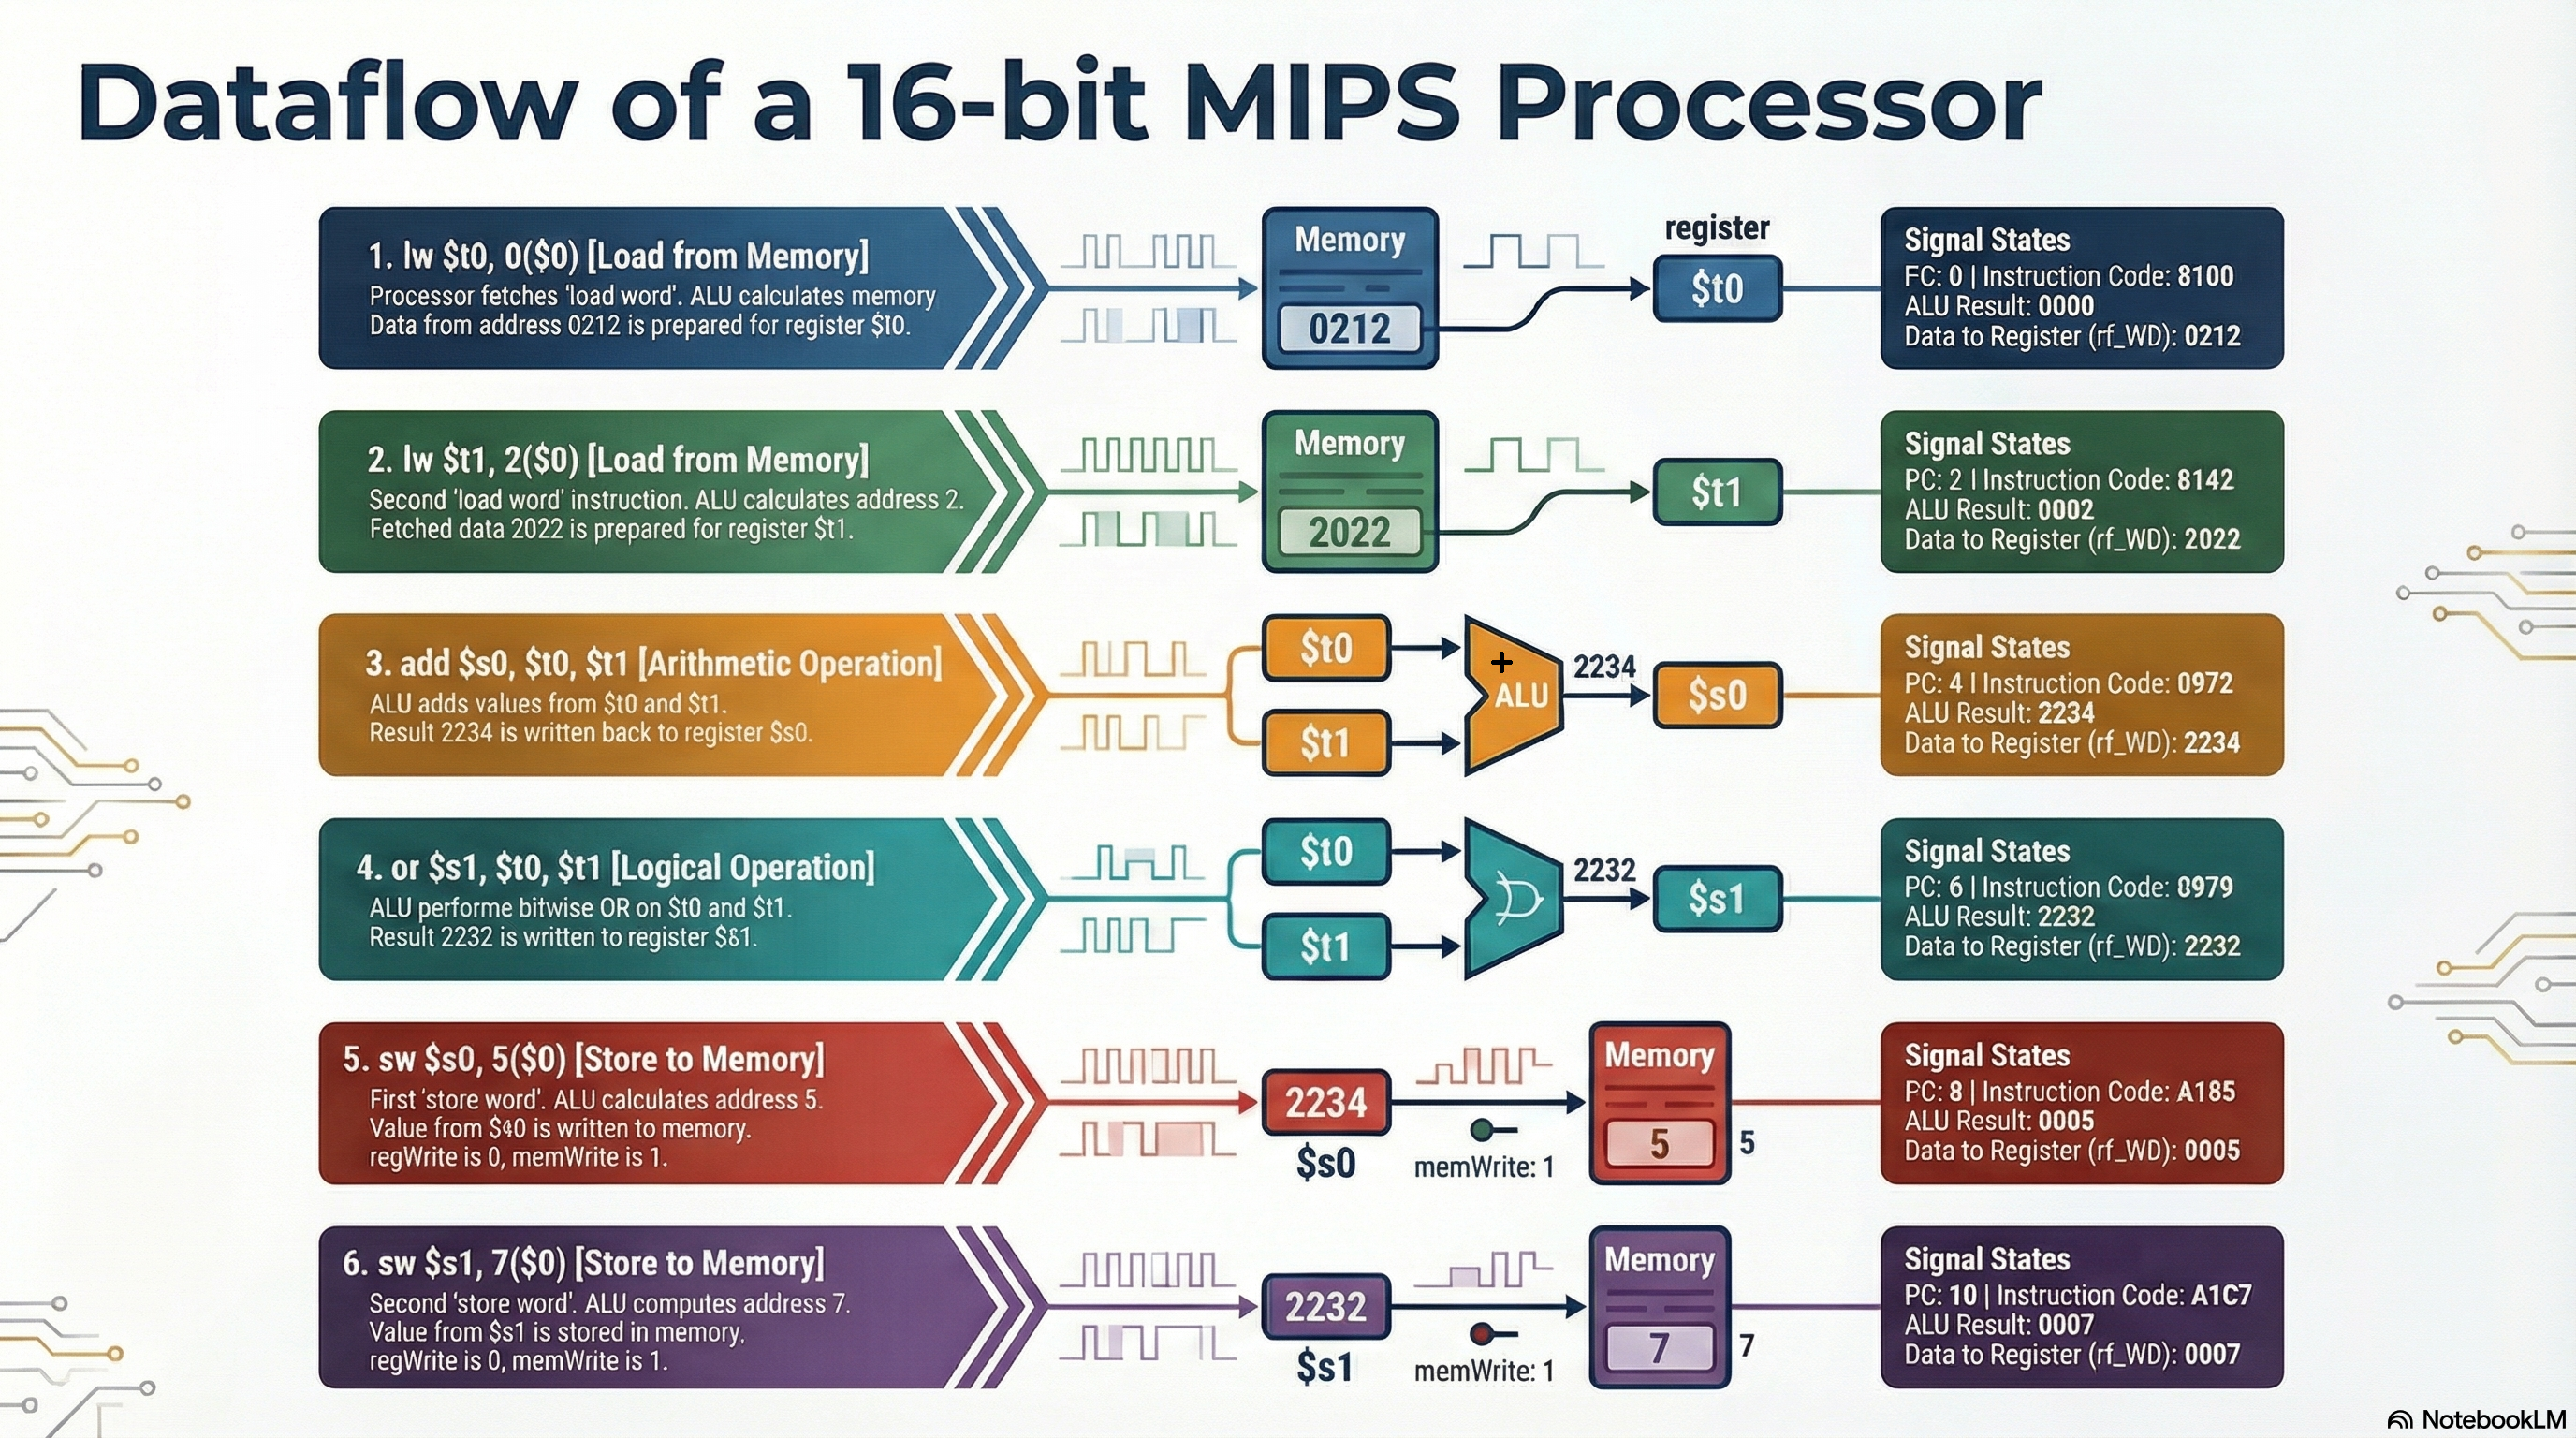
\includegraphics[width=\linewidth]{assets/WaveformSC.png}
        \subcaption{Waveform with annotations}
    \end{minipage}
    \caption{Single-Cycle Simulation Waveform}
    \label{fig:single_cycle_waveform}
\end{figure}

\vspace{0.5cm}

\subsection{Pipelined Verification}
\vspace{0.2cm}
\subsubsection{Pipelined Test Instructions}
\vspace{0.2cm}
The following assembly code was used to test the pipelined processor:
\lstinputlisting[language=Verilog, caption={Pipelined Test Instructions}, label={lst:pipe_instructions}]{assets/codes/Pipe_instructions.asm}

\vspace{0.2cm}

Note that \texttt{nop} instructions were added between actual instructions to avoid \textit{data hazards} in the pipelined architecture (stalling). \textbf{Data hazards} are situations where an instruction depends on the result of a previous instruction that has not yet completed its execution in the pipeline. In this test case, several data hazards were identified that required stalling to ensure correct execution.

\vspace{0.2cm}

The first hazard that is encountered is a \textit{load-use hazard}\footnote{A load-use hazard occurs when an instruction tries to use data that is being loaded by a previous instruction that has not yet completed.} between the \texttt{LW} and \texttt{ADD} instructions. The rest of the hazards are \textit{RAW hazards}\footnote{A read-after-write (RAW) hazard occurs when an instruction depends on the \textbf{result} of a previous instruction that has not yet completed.} between the \texttt{ADDI} and \texttt{SW} instructions.

\vspace{0.3cm}

\subsubsection{Pipelined Simulation Waveform}
\vspace{0.2cm}

\begin{figure}[H]
    \centering
    \begin{minipage}{\linewidth}
        \centering
        \includegraphics[width=\linewidth]{assets/WaveformPipe.jpg}
        % \subcaption{Original waveform}
    \end{minipage}

    % \vspace{1em}

    % \begin{minipage}{\linewidth}
    %     \centering
    %     \includegraphics[width=\linewidth]{assets/WaveformPipe.png}
    %     \subcaption{Waveform with annotations}
    % \end{minipage}
    \caption{Pipelined Simulation Waveform}
    \label{fig:pipelined_waveform}
\end{figure}

\vspace{0.5cm}

\section{Timing Analysis (Performance Comparison)}
\vspace{0.3cm}

\subsection{Timing Analysis Methodology}
\vspace{0.2cm}
\vspace{0.2cm}

Three main metrics were extracted from Quartus timing analysis reports for both architectures:

\vspace{0.2cm}

\begin{itemize}[itemsep=0.1cm]
    \item \textbf{Maximum Frequency (\textrm{F\textsubscript{max}}):} The highest clock frequency at which the processor can operate without timing violations. This metric is reported from the Quartus compilation report.
    \item \textbf{Total Execution Time:} Execution Time $= \mathrm{IC} \ \times \ \mathrm{CPI} \ \times \ \text{Clock Cycle Time}$, where IC is the instruction count, CPI is cycles per instruction, and Clock Cycle Time is $1/F_\mathrm{max}$.
\end{itemize}

\vspace{0.2cm}

For simplicity, no critical path analysis was performed. Instead, the maximum frequency reported by Quartus was used to calculate the clock cycle time for both architectures.

\vspace{0.4cm}

\subsection{Compilation Summary}
\vspace{0.2cm}
\subsubsection{Timing Comparison}
\vspace{0.2cm}
The timing analysis comparison between the single-cycle and pipelined architectures is
summarized in \autoref{tab:timing_comparison}.

\vspace{0.3cm}

\textbf{Performance Metrics:}
\vspace{0.2cm}
\begin{itemize}[itemsep=0.1cm]
    \item \textbf{Maximum Frequency:} Was reported directly from Quartus compilation reports.
    \item \textbf{Clock Cycle Time:} Calculated as the inverse of the maximum frequency.
    \item \textbf{Instruction Count (IC):} Both architectures executed the same number of instructions (6 instructions).
    \item \textbf{Cycles Per Instruction (CPI):} The single-cycle architecture has a CPI of 1, while the pipelined architecture has a CPI of 2.5\footnote{$\mathrm{CPI_{pipe}} = \dfrac{\mathrm{Total\ Cycles}}{\mathrm{Instruction\ Count\ (IC)}} = \dfrac{\mathrm{Pipeline Depth} + N - 1}{6} = \dfrac{15}{6} = 2.5$} due to the inserted stalls (\texttt{nop}) instructions to handle data hazards.
    \item \textbf{Total Execution Time:} Calculated using the formula mentioned in the methodology section.
\end{itemize}

\vspace{0.3cm}

\begin{table}[H]
    \centering
    \begin{tabular}{|l|c|c|}
        \hline
        \textbf{Metric}           & \textbf{Single-Cycle} & \textbf{Pipelined} \\ \hline
        Maximum Frequency (MHz)   & 61.55                 & 93.18              \\ \hline
        Clock Cycle Time (ns)     & 16.25                 & 10.73              \\ \hline
        Instruction Count         & 6                     & 6                  \\ \hline
        Cycles Per Instruction    & 1                     & 2.5 (with stalls)  \\ \hline
        Total Execution Time (ns) & 97.5                  & 160.98             \\ \hline
    \end{tabular}
    \caption{Timing Analysis Comparison}
    \label{tab:timing_comparison}
\end{table}

\vspace{0.4cm}

\subsection{Performance Comparison Summary}
\vspace{0.2cm}

The pipelined processor exhibits a 65\% increase in execution time (160.98 ns vs. 97.5 ns) despite a 51\% higher clock frequency. This counterintuitive result stems from the absence of hazard detection and data forwarding mechanisms.

\textbf{Root Cause:} The 6 useful instructions require 5 manual \texttt{nop}s to resolve data hazards:
\vspace{0.2cm}
\begin{itemize}[itemsep=0.1cm]
    \item 3 NOPs for load-use hazards (after \texttt{lw} instructions)
    \item 2 NOPs for RAW hazards (before \texttt{sw} instructions to wait for \texttt{\$s0}/\texttt{\$s1} writes)
\end{itemize}

\vspace{0.3cm}

\textbf{Performance Impact:}
\vspace{0.2cm}
\begin{itemize}[itemsep=0.1cm]
    \item CPI increases from 1.0 to 2.5 (150\% penalty)
    \item Pipeline efficiency: 54.5\% (6 useful / 11 total instructions)
    \item Speedup: $\frac{97.5}{160.98} = 0.606$ (39.4\% performance loss)
\end{itemize}

\vspace{0.5cm}

\section{Conclusion}
\vspace{0.3cm}

This report presented the design and implementation of a 16-bit MIPS processor in both single-cycle and pipelined architectures. The processor implements a 12-instruction ISA with separate 64-byte instruction and data memories in little-endian format, an 8-register file, and complete datapath components including PC, control unit, ALU, sign extension, and multiplexers. The single-cycle design executes each instruction in one clock cycle with straightforward control flow, while the pipelined architecture divides execution into five stages (IF, ID, EX, MEM, WB) separated by pipeline registers to enable instruction overlap.

Both designs were verified through waveform simulations. The performance analysis revealed that without hazard detection and data forwarding mechanisms, the pipelined processor exhibited 65\% longer execution time despite higher clock frequency, requiring manual \texttt{nop} insertions that increased CPI from 1.0 to 2.5. This demonstrates that pipelining benefits are only realized with proper hazard management.

Future work should include implementing forwarding units, hazard detection hardware, branch prediction, an expanded instruction set, and larger memory spaces to fully leverage pipelined execution advantages.


\end{document}